\documentclass[12pt,letterpaper, onecolumn]{exam}
\usepackage{amsmath}
\usepackage{amssymb}
\usepackage{amsthm}
\usepackage{graphicx}
\usepackage{mathrsfs}
\usepackage{xcolor}
\usepackage[lmargin=71pt, tmargin=1.2in]{geometry}  %For centering solution box
\usepackage[english]{babel}
\newtheorem{theorem}{Theorem}
\newtheorem{lemma}[theorem]{Lemma}
\usepackage{accents}
\usepackage{ulem} % sout() to crossing things out 
\newcommand{\ubar}[1]{\underaccent{\bar}{#1}}
\newcommand{\bs}[1]{\boldsymbol{#1}}
\newcommand{\bm}[1]{\mathbf{#1}}
\newcommand{\der}[2]{\frac{d #1}{d#2}}
\newcommand{\pder}[3]{\frac{\delta^{#3} #1}{\delta^{#3}#2}}
\newcommand{\rs}{$X_1, ..., X_n$}
\newcommand{\nsum}{\sum_{i=1}^n}
\newcommand{\nprod}{\prod_{i=1}^n}
\newcommand*{\Comb}[2]{{}^{#1}C_{#2}}%
\newcommand{\ifc}{\textrm{ if }}
\newcommand{\real}{\mathbb{R}}
\newcommand{\nat}{\mathbb{N}}
\newcommand{\power}{\mathcal{P}}
\newcommand{\rational}{\mathbb{Q}}
\newcommand{\cutelim}{\lim\limits_{n\to\infty}}
\newcommand{\salg}{$\sigma$-algebra }

\newcommand{\calA}{\mathcal{A}}
\newcommand{\calO}{\mathcal{O}}
\newcommand{\calC}{\mathcal{C}}
\newcommand{\calB}{\mathcal{B}}
\newcommand{\calI}{\mathcal{I}}
\newcommand{\calF}{\mathcal{F}}
\newcommand{\calG}{\mathcal{G}}
\newcommand{\gensig}[1]{\sigma\langle #1 \rangle} % notation for a sigma algebra generated by some set 
\newcommand{\om}{\mu^*} % outer measure 
\newcommand{\rat}{\mathbb{Q}}
\newcommand{\tribrac}[1]{\langle #1 \rangle}
\newcommand{\borel}{\mathcal{B}(\mathbb{R})}
\newcommand{\boreltwo}{\mathcal{B}(\mathbb{R}^2)}
\newcommand{\borelk}[1]{\mathcal{B}(\mathbb{R}^#1)}
\newcommand{\probspace}{(\Omega, \calF, P)}

\newcommand{\Iunion}{\bigcup_{\alpha \in I}}
\newcommand{\Iintersect}{\bigcap_{\alpha \in I}}

\newcommand{\dm}{d \mu}

\newcommand{\cutesum}[1]{\sum_{#1 = 1}^\infty}

\newcommand{\nti}{n \to \infty}


% \chead{\hline} % Un-comment to draw line below header
\thispagestyle{empty}   %For removing header/footer from page 1

\begin{document}

\begingroup  
    \centering
    \LARGE STAT 6410\\
    \LARGE Homework 6\\[0.5em]
    \large Sarah Kilgard\par
\endgroup
\rule{\textwidth}{0.4pt}
\pointsdroppedatright   %Self-explanatory
\printanswers
\renewcommand{\solutiontitle}{\noindent\textbf{Ans:}\enspace}   %Replace "Ans:" with starting keyword in solution box

\begin{questions}
%%%%%%%%%%% Question 1 %%%%%%%%%%%%%%%%%%%%    
    \question \textbf{Chapter 2, Problem 28}

    Let $\mu$ be the Lebesgue measure on $([-1, 1], \calB([-1, 1]))$. For $n \geq 1$, define $f_n(x) = n I_{(0, n^{-1})}(x) - n I_{(-n^{-1}, 0)}(x)$ and $f(x) \equiv 0$ for $x \in [-1, 1]$. Show that $f_n \to f$ a.e. $\mu$ and $\int f_n d\mu \to \int f d\mu$ but $\{f_n\}_{n \geq 1}$ is not UI.
    \begin{solution}
        \begin{proof}
            For each $x \in [-1,1]$, there exists some $N \in \nat$ such that $x \notin (-n^{-1}, n^{-1})$.

            Thus, for all sufficiently large $n \geq N$, $f_n(x) = 0$. Thus, $\lim\limits_{n \to \infty} f_n(x) = f(x)$ for all $x \in [-1, 1].$ Since this is true for all $x \in [-1, 1]$, and $\mu([-1, 1]^c) = \mu(\emptyset) = 0$, $f_n \to f$ a.e.$(\mu)$.

            \begin{align*}
                & \lim\limits_{n \to \infty} \int f_n d\mu = \lim\limits_{n \to \infty} (n \mu(0, n^{-1}) - n \mu(-n^{-1}, 0)) = 0 - 0 = 0 \\
                & \int f d\mu = 0 \\
                & \therefore \: \int f_n d\mu \to \int f d\mu
            \end{align*}

            Let $t > 0$ be given.
            $\sup_{n \geq 1} \int_{|f_n| > t} |f_n| d\mu = 2$

            Thus, $\{f_n\}_{n \geq 1}$ is not uniformly integrable.
        \end{proof}
    \end{solution}

%%%%%%%%%%% Question 2 %%%%%%%%%%%%%%%%%%%%    
    \question \textbf{Chapter 2, Problem 30}

    For $n \geq 1$, let $f_n(x) = n^{-1/2}I_{(0, n)}(x), \: x \in \real$ and let $f(x) \equiv 0$. Let $m$ denote the Lebesgue measure on $(\real, \borel)$. Show that $f_n \to f$a.e.$(m)$ and $\{f_n\}_{n\geq1}$ is UI, but $\int f_n dm \not\to \int f dm$
    \begin{solution}
        \begin{proof}
            \textbf{WTS:} $f_n \to f a.e.(m)$ \\
            
            \begin{align*}
                & B = \{x \in \real: \cutelim f_n(x) \neq f(x)\} \\
                & = \{x \in \real: \cutelim n^{-1/2}I_{(0, n)}(x) \neq 0\} \\
                & \textrm{Since } \cutelim n^{-1/2} = 0, \: B = \emptyset \\
                & m(\emptyset) = 0 \: \implies \: f_n \to f a.e.(m)
            \end{align*}

            \textbf{WTS:} $\int f_n dm \not\to \int f dm$

            $\int f dm = \int 0 dm = 0$

            $\cutelim f_n(x) dm(x) = \cutelim (m((0, n)^c) \times 0 + m((0, n)) \times n^{-1/2}) = 0 + \cutelim (\frac{n}{\sqrt{n}}) = \cutelim(\sqrt{n}) \neq 0$. 

            Thus, $\int f_n dm \not\to \int f dm$.
        \end{proof}
    \end{solution}
        
%%%%%%%%%%% Question 3 %%%%%%%%%%%%%%%%%%%%    
    \question \textbf{Chapter 2, Problem 36}

    \begin{itemize}
        \item[(a)] Let $\{f_n\}_{n \geq 1} \subset L^1(\Omega, \calF, \mu)$ such that $f_n \to 0$ in $L^1(\mu)$. Show that $\{f_n\}_{n\geq1}$ is UI.
        \item[(b)] Let $\{f_n\}_{n \geq 1} \subset L^p(\Omega, \calF, \mu), \: 0 < p < \infty$, such that $\mu(\Omega) < \infty$, $\{|f_n|^p\}_{n\geq1}$ is UI, and $f_n \to^m f$. Show that $f \in L^p(\mu)$ and $f_n \to f$ in $L^p(\mu).$
    \end{itemize}
    
    \begin{figure}[h!]
        \centering
        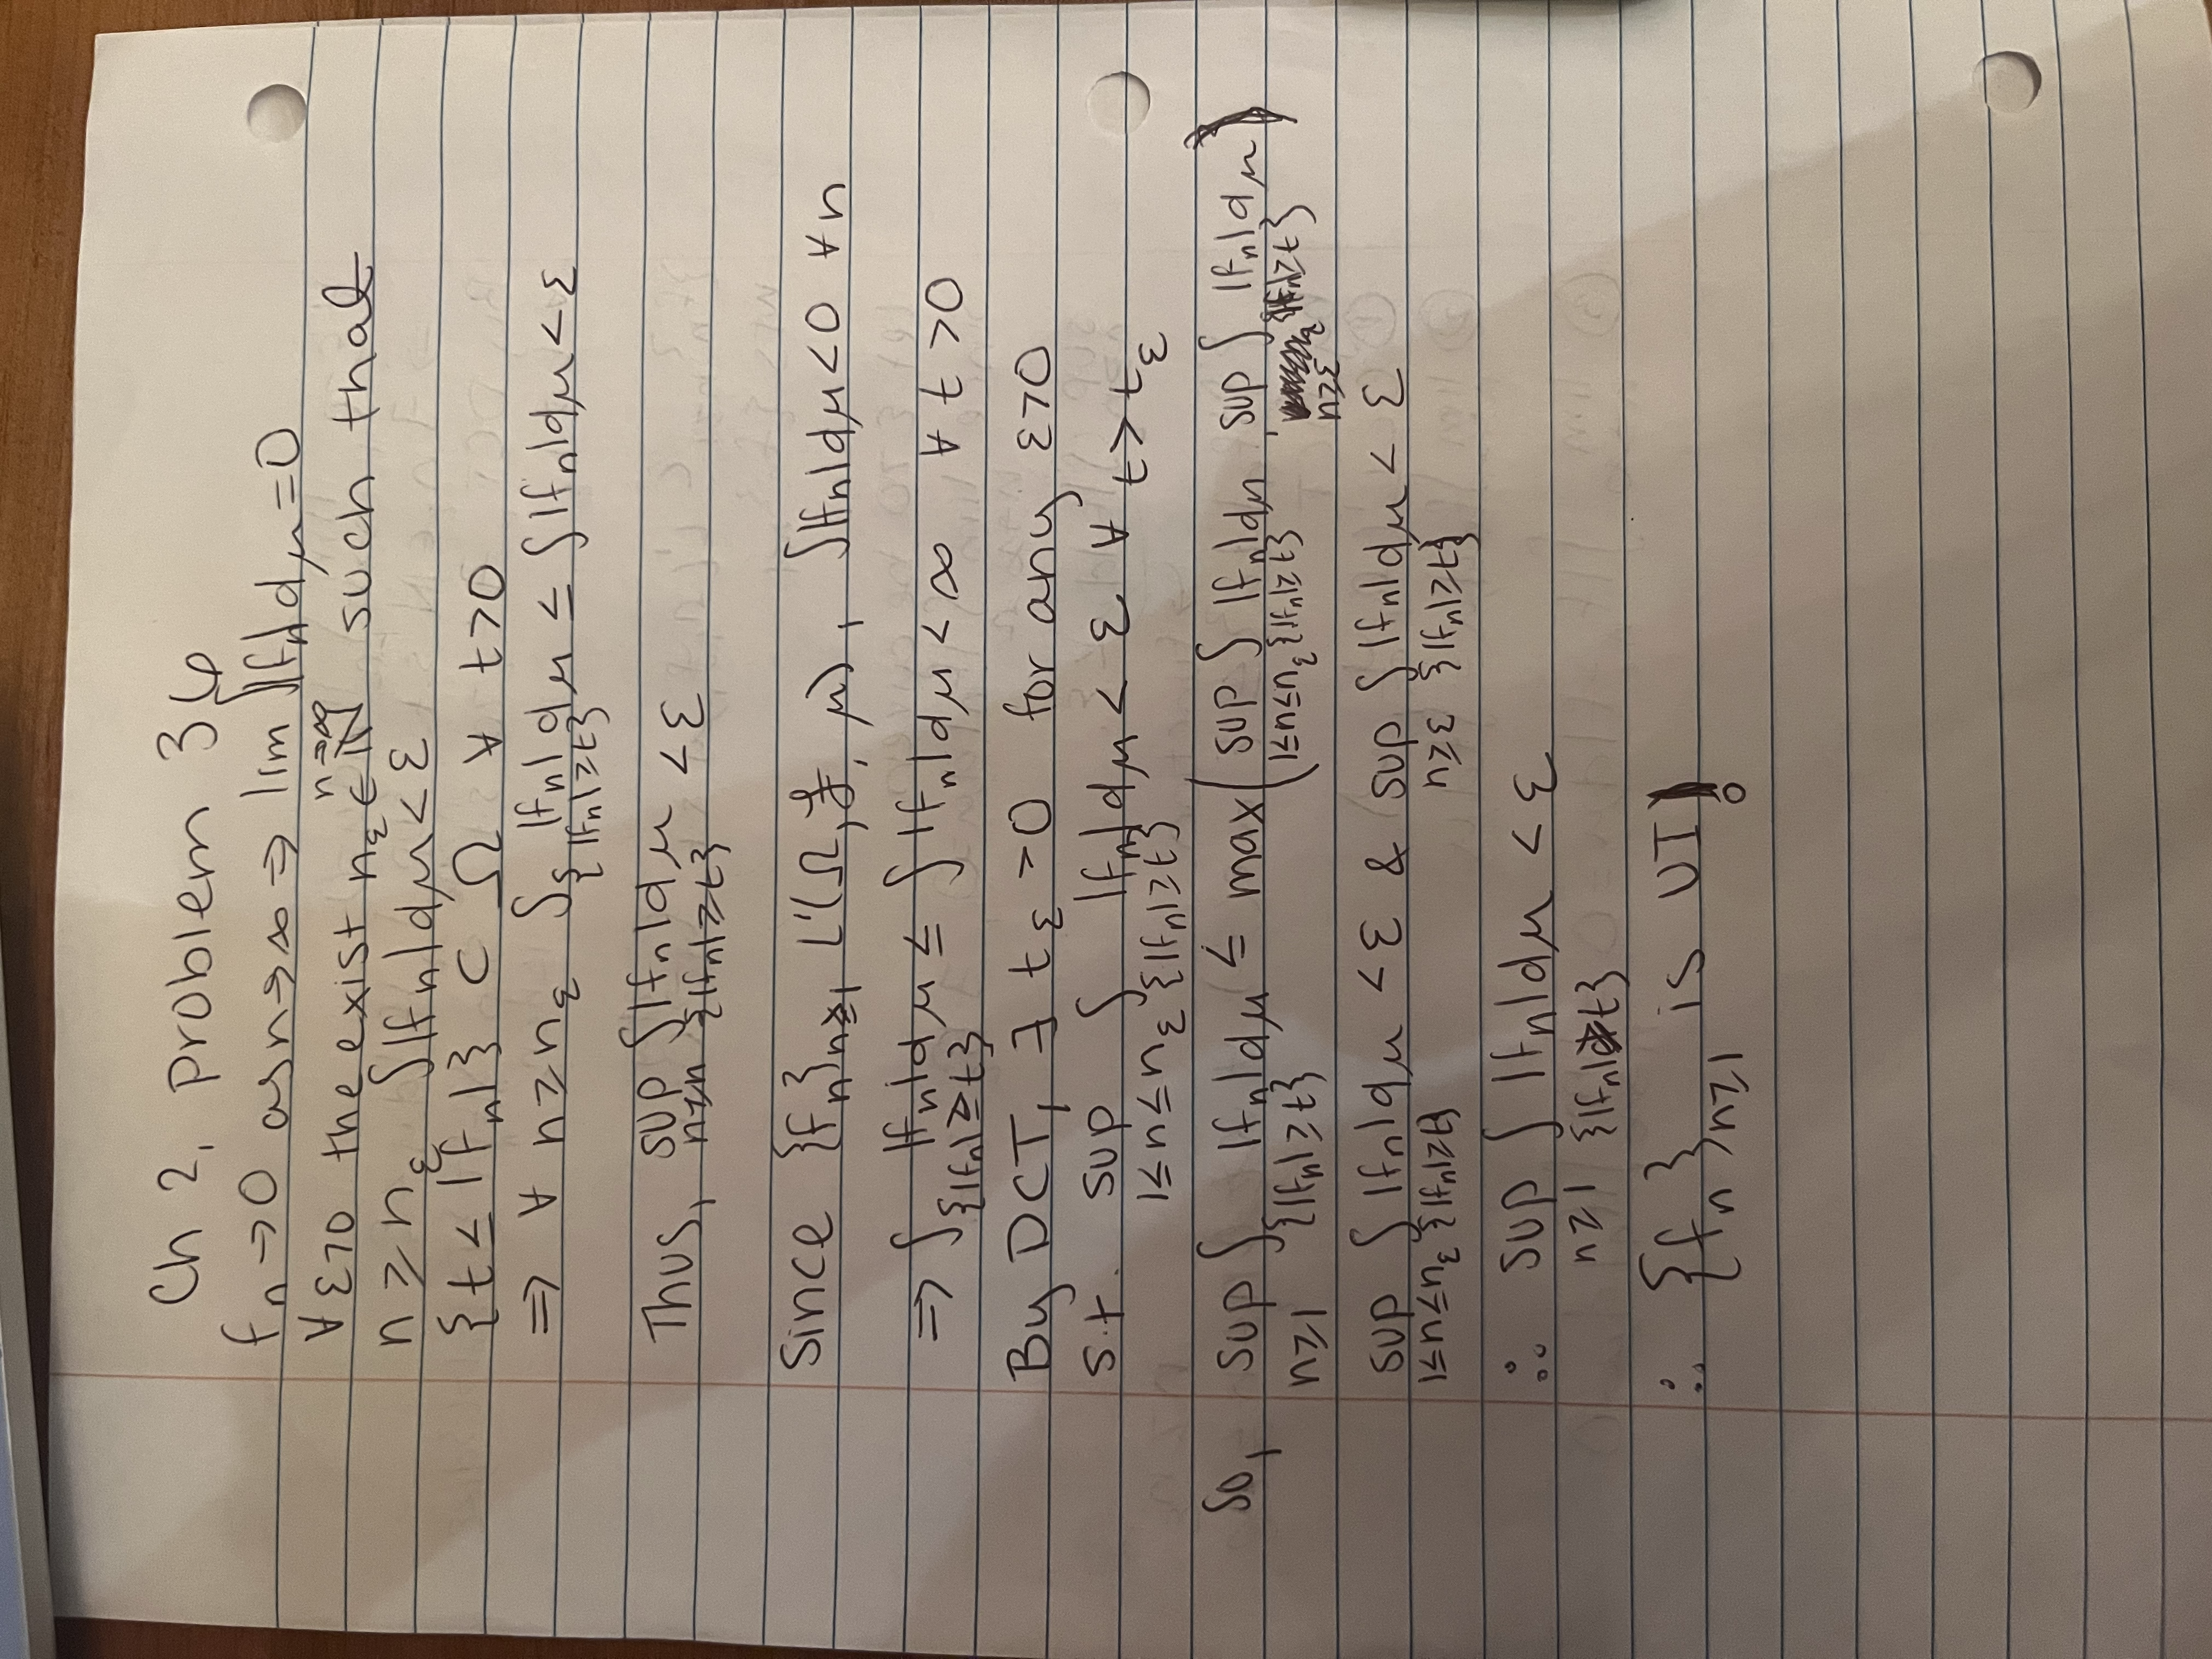
\includegraphics[width=1\linewidth]{images/ch2.36a.png}
    \end{figure}
Note: I don't know how to fix the orientation. 
(a) Is on the next page.
(b) I'm quite confused about this one, to be honest. 
    
\newpage 

%%%%%%%%%%% Question 4 %%%%%%%%%%%%%%%%%%%%    
    \question \textbf{Chapter 2, Problem 42}

    (\textit{Change of variables formula}) Let $(\Omega_i, \calF_i)$, $i = 1, 2$ be two measurable spaces. Let $f: \Omega_1 \to \Omega_2$ be $\tribrac{\calF_1, \calF_2}$-measurable, $h: \Omega_2 \to \real$ be $\tribrac{\calF_2, \borel}$-measurable, and $\mu_1$ be a measure on $(\Omega_1, \calF_1)$. Show that $g \equiv h \circ f$, i.e., $g(\omega) \equiv h(f(\omega))$ for $\omega \in \Omega_1$ is in $L^1(\mu)$ iff $h(\cdot) \in L^1(\Omega_2, \calF_2, \mu_2)$ where $\mu_2 = \mu_1 f^{-1}$ iff $I(\cdot) \in L^1(\real, \borel, \mu_3 \equiv \mu_2h^{-1})$ where $I(\cdot)$ is the identity function in $\real$, i.e., $I(x) \equiv x$ for all $x \in \real$ and also that:
    \[\int_{\Omega_1} g d\mu_1 = \int_{\Omega_2} h d\mu_2 = \int_{\real} x d\mu_3\]

    Hint: to show the first equality (and the first part of the problem), start with a simple non-negative function $h$ and follow the usual steps to conclude about general $h$. The second part of the problem is related to the first part.

    the work is at the bottom of this document. 
    
    \begin{figure}[h!]
        \centering
        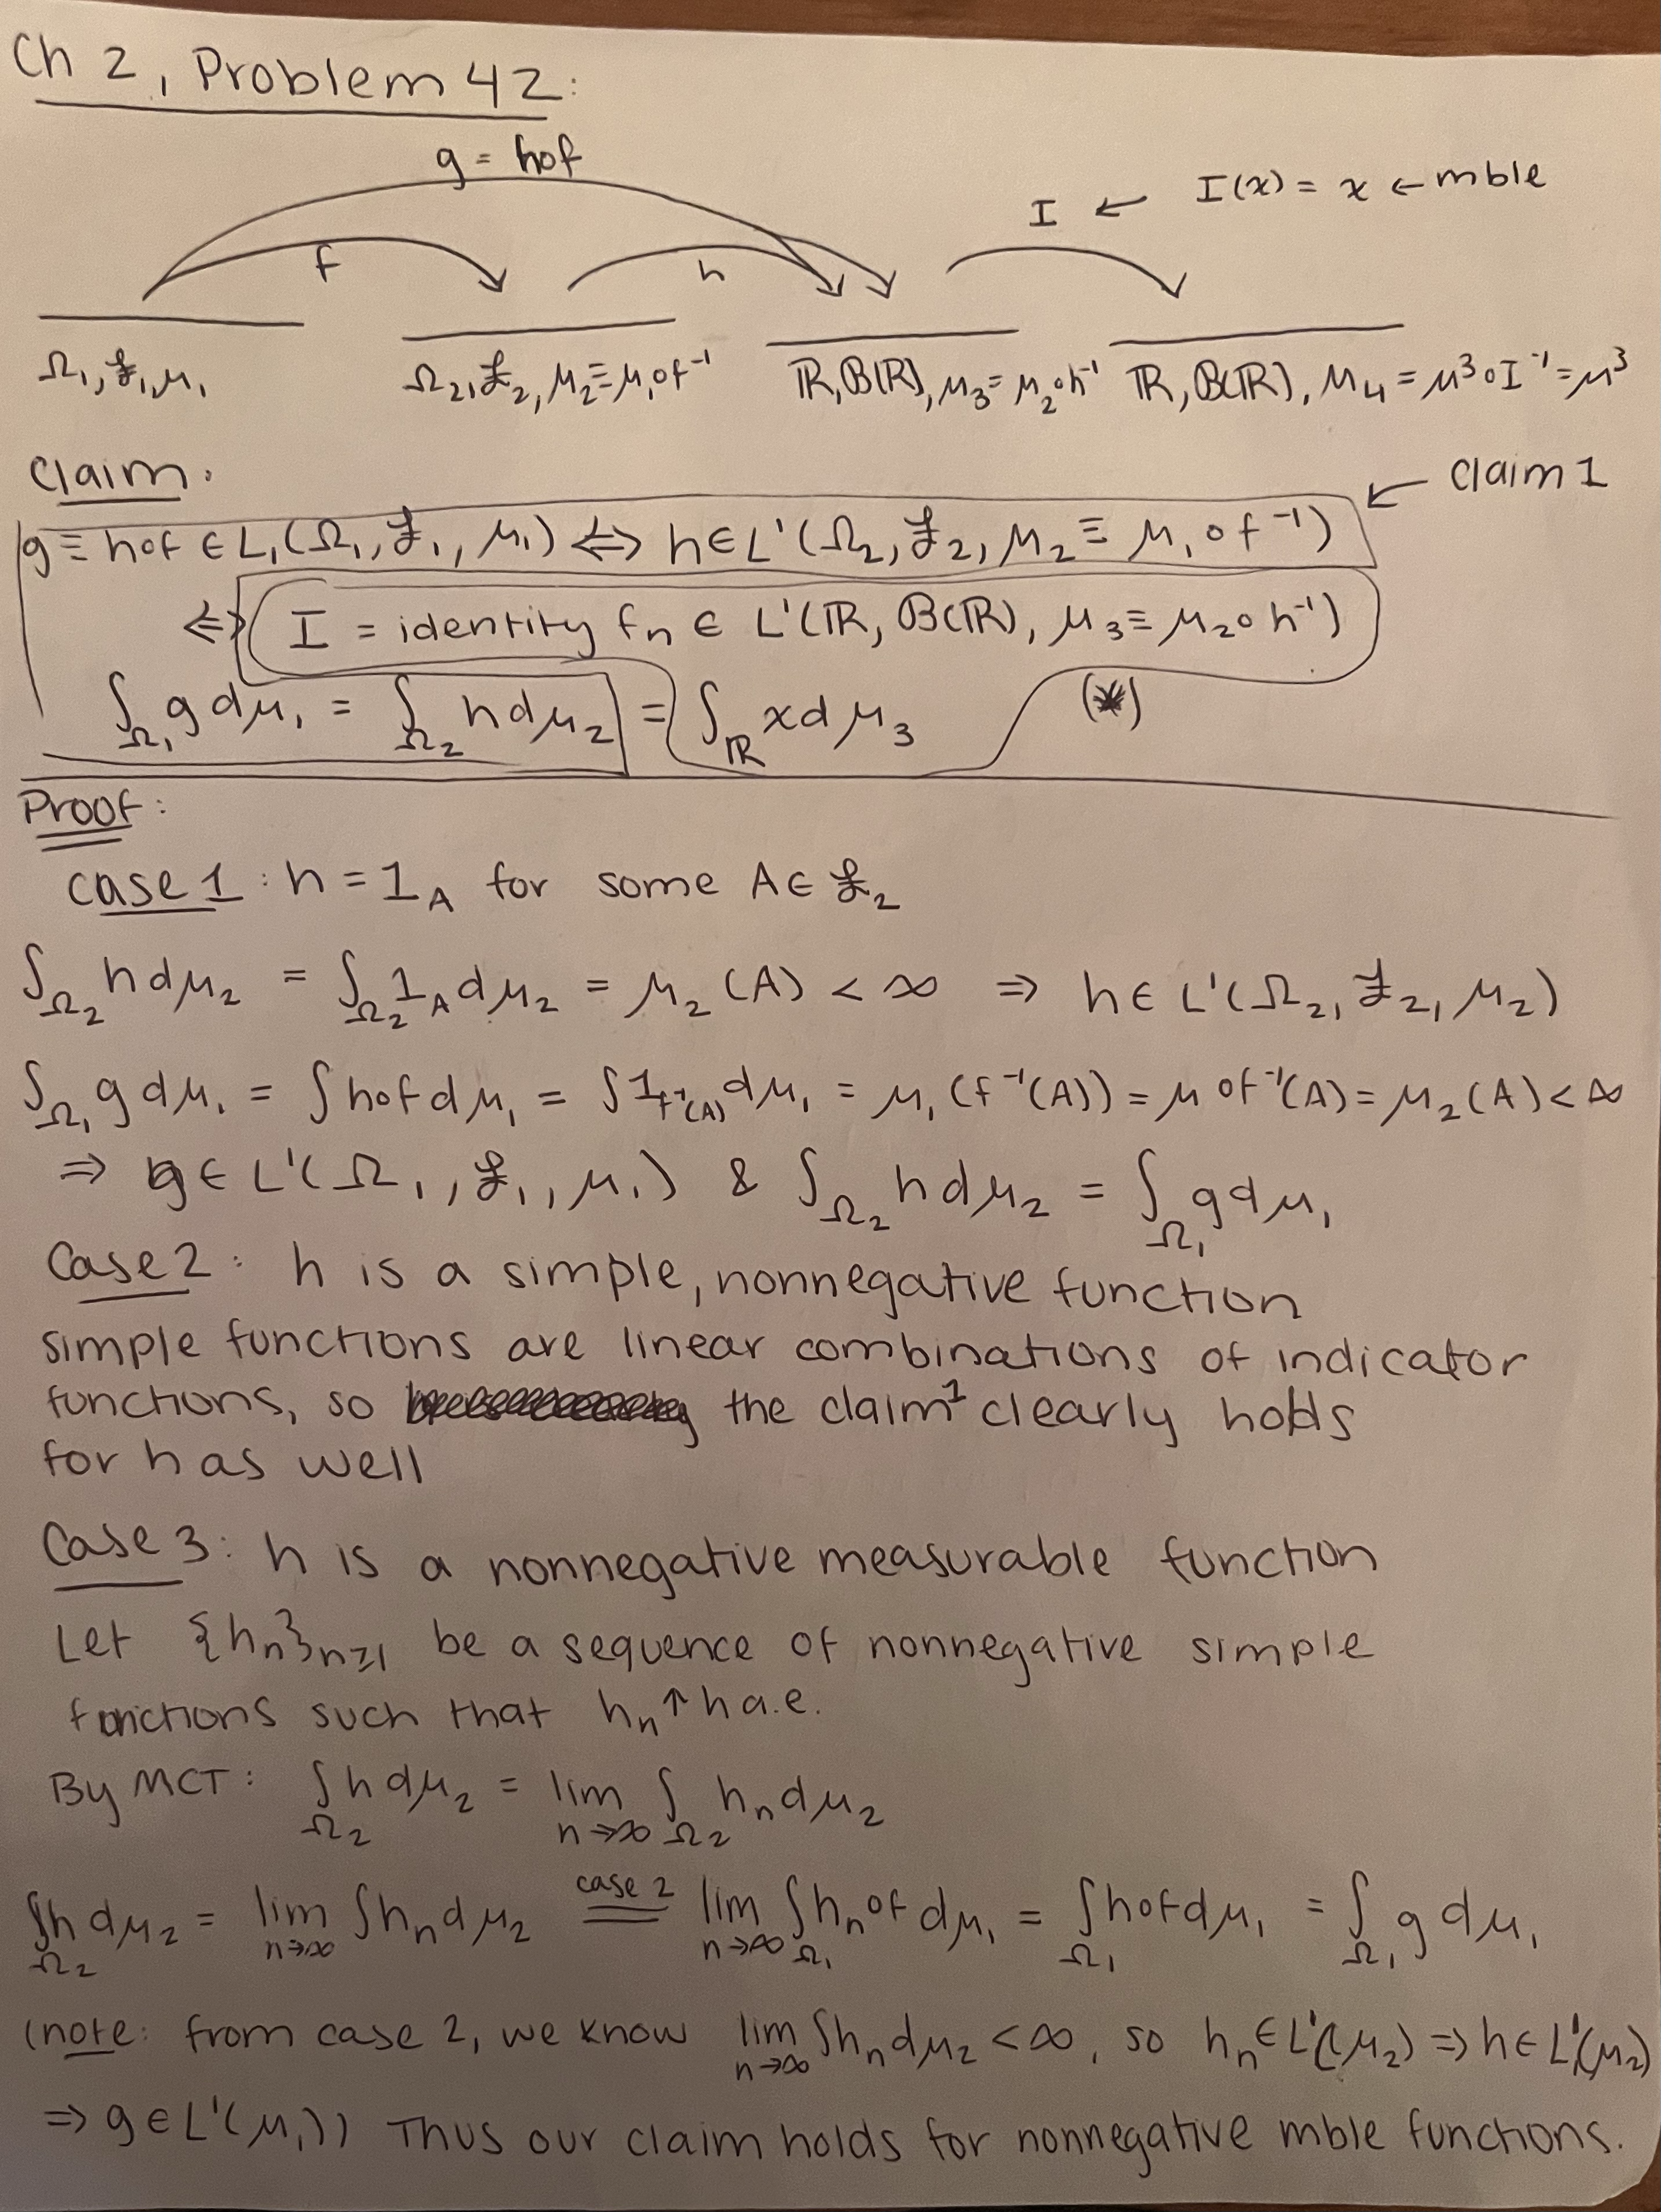
\includegraphics[width=1\linewidth]{images/hw6.q4.p1.png}
    \end{figure}
    \begin{figure}[h!]
        \centering
        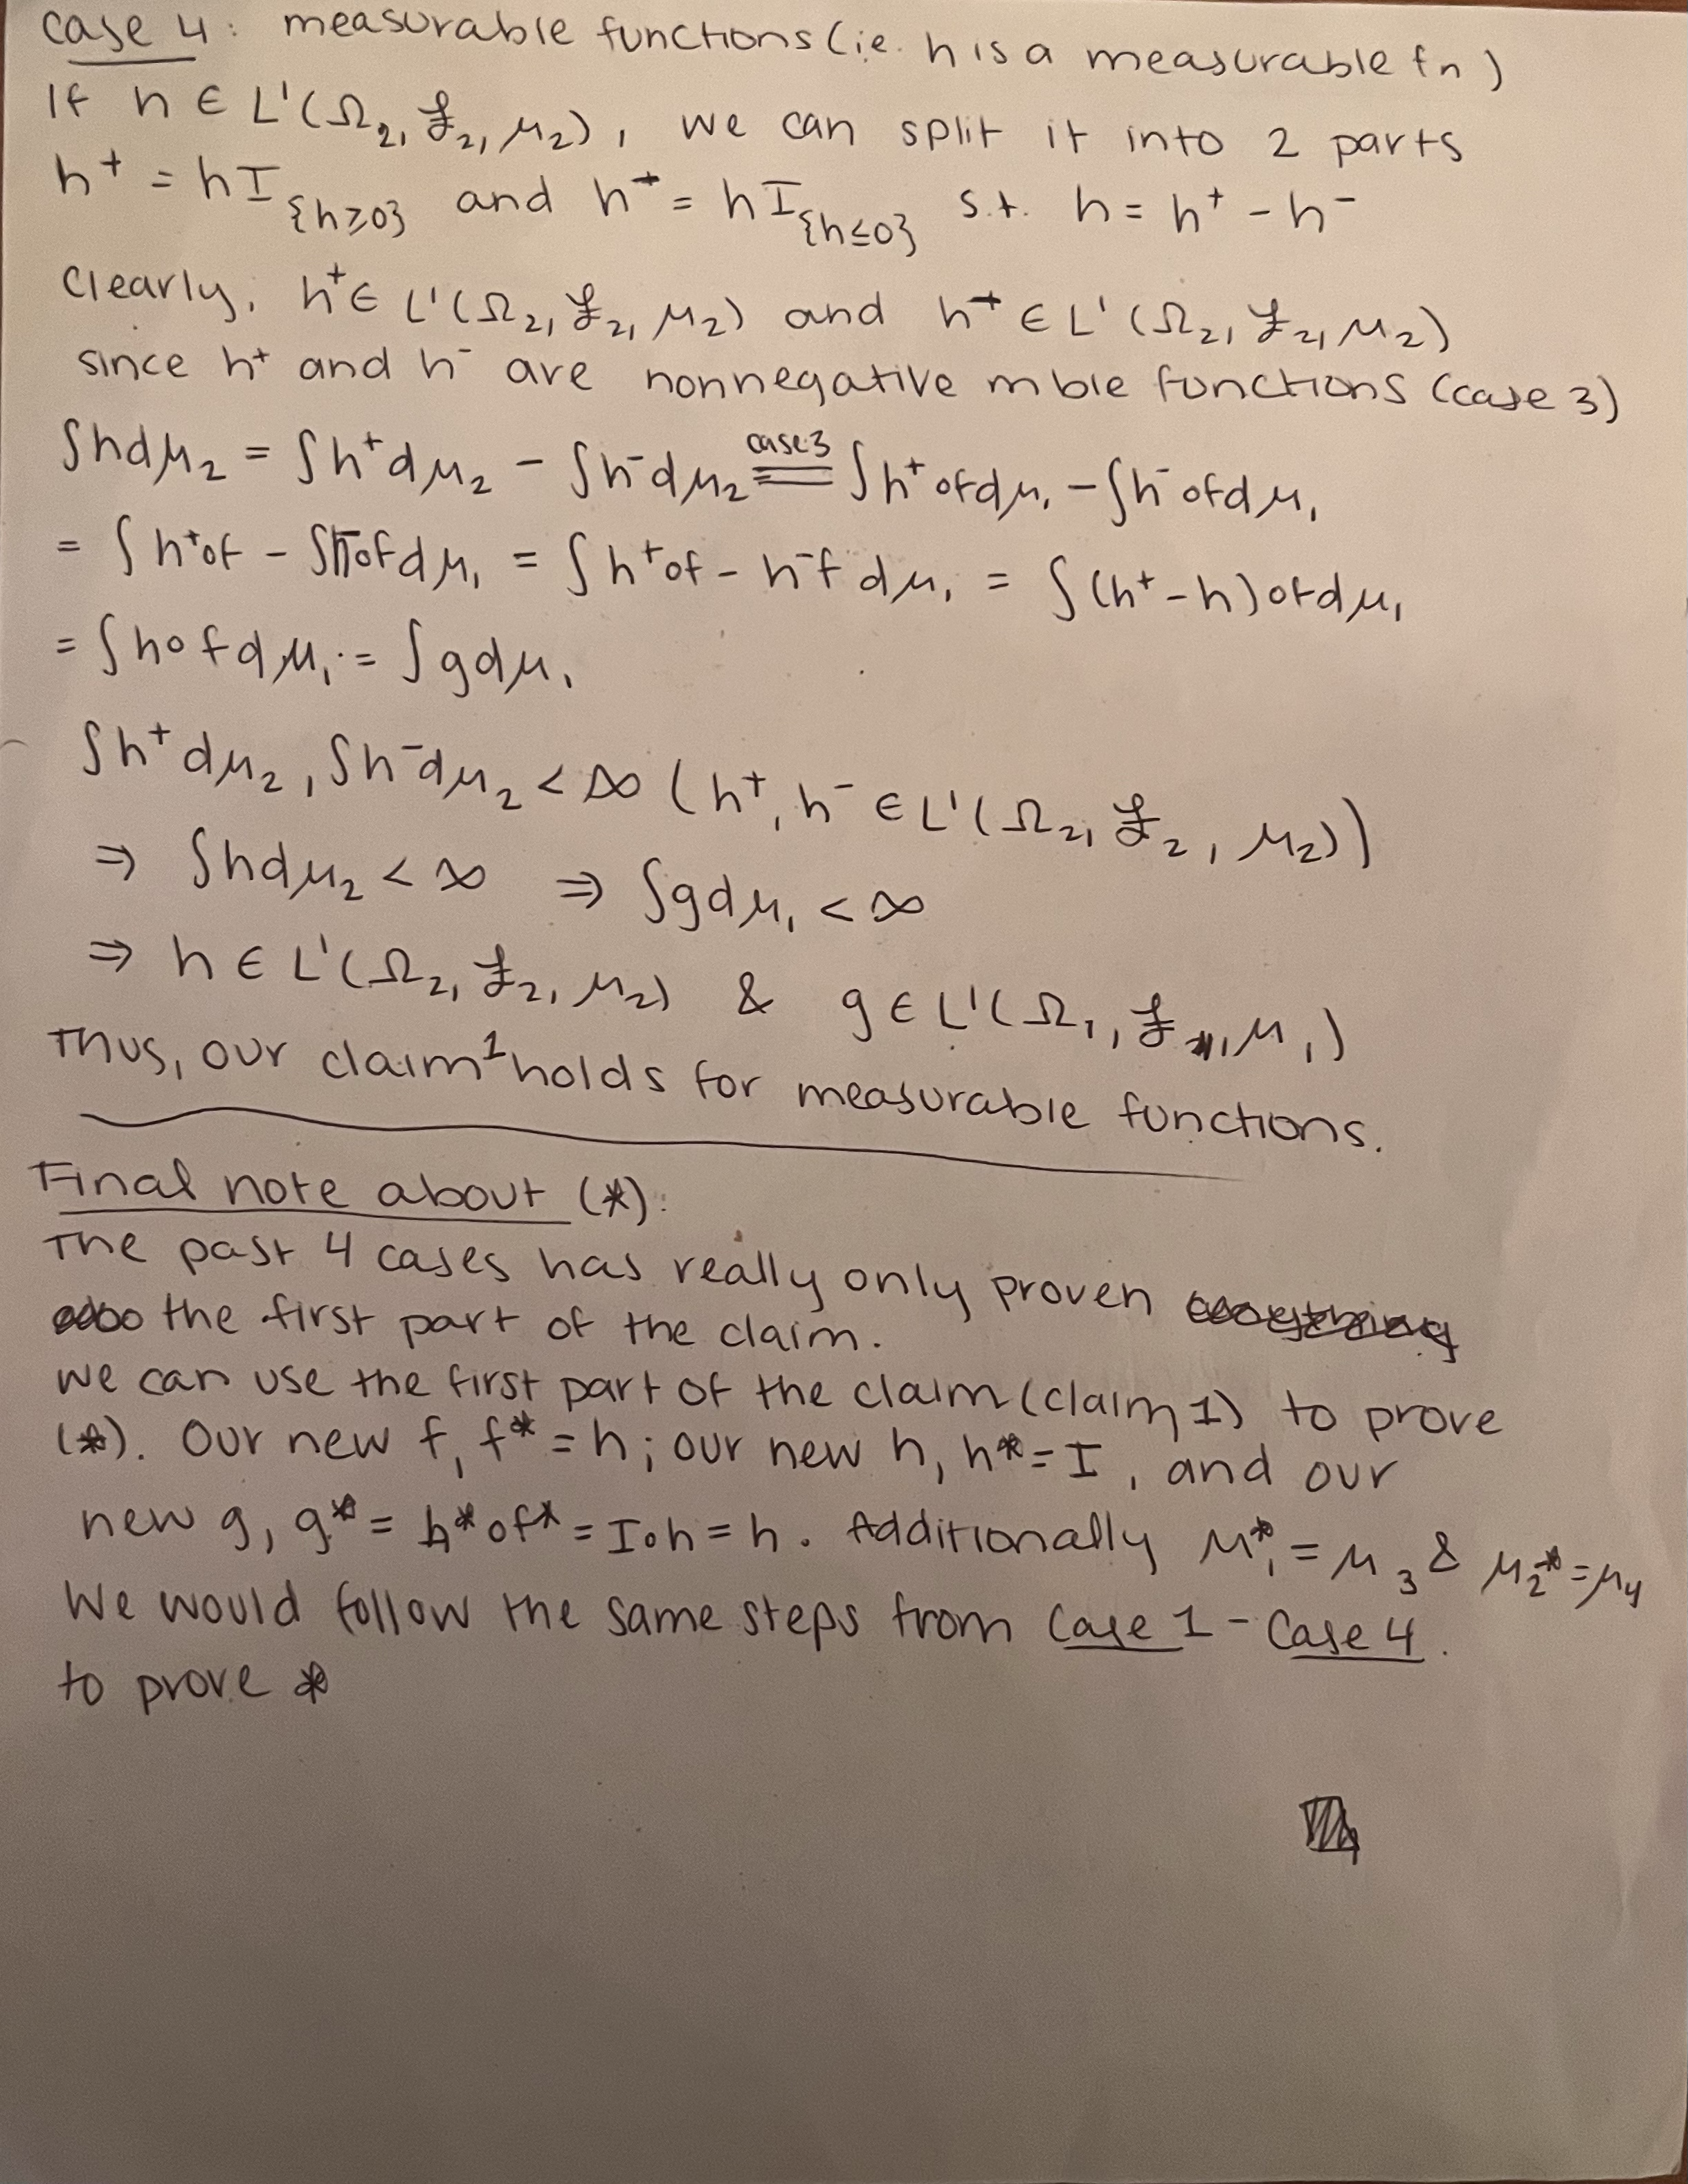
\includegraphics[width=1\linewidth]{images/hw6.q4.p2.png}
    \end{figure}

\newpage

%%%%%%%%%%% Question 5 %%%%%%%%%%%%%%%%%%%%    
    \question \textbf{Additional Problem A:}

    Let $(\Omega, \calF, P) = ([0, 1], \calB([0, 1]), m)$, where $m$ denotes the Lebesgue measure. Define the random variables $X, \: \{X_n\}:$ for each $\omega \in \Omega$, $X(\omega) = 1$
    \[X_1(\omega) = 0, \: X_n(\omega) = 1 + (n - 1)\mathbf{I}_{\{[0, \frac{1}{n}]\}}(\omega), \: n \geq 2\]
    \begin{itemize}
        \item[(a)] Does $X_n \to X$ \textit{everywhere} as $n \to \infty$?
        \item[(b)] Does $X_n \to X$ a.s.(P) as $\nti$? 
        \item[(c)] Does $X_n \to X$ in probability as $\nti$?
        \item[(d)] Does $X_n \to X$ in $L^p$ as $\nti$? Argue for different values of $p \in (0, \infty)$. 
        \item[(e)] Is $\{X_n\}$ a uniformly integrable sequence of random variables? 
    \end{itemize}
    \begin{solution}
        \begin{itemize}
            \item[(a)] No! Below is a counterexample \begin{proof}
                \begin{align*}
                    & \textrm{If } \omega = 0, \: \cutelim X_n(\omega) = \cutelim X_n(0) = \cutelim(1 + (n - 1)\mathbf{I}_{[0, \tfrac{1}{n}]}(0)) \\
                    & = \cutelim 1 + n - 1 = \cutelim n = \infty \neq 1 = X(0) \\ 
                \end{align*}
            \end{proof}
            
            \item[(b)] \begin{proof}
                \begin{align*}
                    & B = \{\omega \in [0, 1]: \cutelim X_n \neq X\} \\
                    & = \{ \omega \in [0, 1]: \cutelim 1 + (n-1) \mathbf{I}_{[0, \tfrac{1}{n}]}(\omega) \neq 1 \} \\
                    & = \{ \omega \in [0, 1]: \cutelim (n-1) \mathbf{I}_{[0, \tfrac{1}{n}]}(\omega) \neq 0 \} \\
                    & \textrm{For each } \omega \in (0, 1] \: \exists N_\omega \in \nat \: s.t. \: \omega > \frac{1}{N_\omega} \\
                    & \textrm{Clearly, as } \nti \: n \textrm{ will surpass } N_\omega \\
                    & \textrm{When } n > N_\omega, \: \omega\notin [0, \tfrac{1}{n}] \: \implies \: \mathbf{I}_{[0, \tfrac{1}{n}]}(\omega) = 0 \\
                    & \therefore \: \cutelim (n - 1) \mathbf{I}_{[0, 1]}(\omega) = 0 \: \forall \: \omega \in (0, 1] \\
                    & \textrm{If } \omega = 0, \: \cutelim((n - 1)\mathbf{I}_{[0, \tfrac{1}{n}]}(0)) \\
                    & = \cutelim n - 1 = \infty \neq 0 \\ 
                    & \textrm{Therefore } B = \{0\}. \\
                    & P(\{0\}) = 0 \: \implies \: X_n \to X \: a.s.(P) \textrm{ as } \nti 
                \end{align*}
            \end{proof}
            \item[(c)] Since $P = m$ is a probability measure $P(\Omega) = 1 < \infty$. Thus, $X_n \to X a.s.(P)$ as $\nti$ $\implies$ $X_n \to X$ in probability as $\nti$.
            \item[(d)] 
            \textbf{For $p = 1$}
            \begin{proof}
                We know from (b) that $X_n \to X  a.s(P)$. \\
                $X$ is a constant function so it is clearly measurable. \\
                For each n, $X_n$ is a linear combination of a constant function ($1$), and an indicator function $\mathbf{I}_{[0, \tfrac{1}{n}]}$, it is a measurable function \\
                Thus, $\{X_n\}_{n \geq 1}$ is a sequence of measurable functions. \\
                $\int X dm = \int 1 \mathbf{I}_{[0,1]} dm = 1 m([0, 1]) = 1 < \infty$ \\
                $\int X_n dm = \int 1 \mathbf{I}_{[0,1]} + (n-1)\mathbf{I}_{[0, \tfrac{1}{n}]} dm \\ = 1m([0, 1]) + (n-1)m([0, \tfrac{1}{n}])= 1 + (n -1)\tfrac{1}{n} = 2 - \tfrac{1}{n} < \infty$ \\
                Thus, by Scheffe's theorem, $X_n \to^{L_1} X$
            \end{proof}
            \textbf{For $0< p< 1$:}\begin{proof}
                Since, $X_n \to^{L_1} X$, $X_n \to^{L_p} X$
            \end{proof}
            \textbf{For $1 < p < \infty$:} \begin{proof}
                For any $\epsilon > 0$, as $\nti$, $\int |X_n|^{1+\epsilon}dm = \int X_n^{1 + \epsilon} dm = \infty$ \\
                Thus, $X_n \not\to^{L_p} X$ when $1 < p < \infty$. 
            \end{proof} 
        \item[(e)]  
        From (d), we know that $X_n \in L^1([0, 1], \mathcal{B}([0, 1]), m)$ that $X_n \to^{L^1(\mu)} X$. Thus, $\{X_n\}_{n \geq 1}$ is UI by Problem 2.36.
        \end{itemize}
    \end{solution}

\end{questions}

\end{document}